% Options for packages loaded elsewhere
\PassOptionsToPackage{unicode}{hyperref}
\PassOptionsToPackage{hyphens}{url}
%
\documentclass[
]{article}
\usepackage{amsmath,amssymb}
\usepackage{lmodern}
\usepackage{iftex}
\ifPDFTeX
  \usepackage[T1]{fontenc}
  \usepackage[utf8]{inputenc}
  \usepackage{textcomp} % provide euro and other symbols
\else % if luatex or xetex
  \usepackage{unicode-math}
  \defaultfontfeatures{Scale=MatchLowercase}
  \defaultfontfeatures[\rmfamily]{Ligatures=TeX,Scale=1}
\fi
% Use upquote if available, for straight quotes in verbatim environments
\IfFileExists{upquote.sty}{\usepackage{upquote}}{}
\IfFileExists{microtype.sty}{% use microtype if available
  \usepackage[]{microtype}
  \UseMicrotypeSet[protrusion]{basicmath} % disable protrusion for tt fonts
}{}
\makeatletter
\@ifundefined{KOMAClassName}{% if non-KOMA class
  \IfFileExists{parskip.sty}{%
    \usepackage{parskip}
  }{% else
    \setlength{\parindent}{0pt}
    \setlength{\parskip}{6pt plus 2pt minus 1pt}}
}{% if KOMA class
  \KOMAoptions{parskip=half}}
\makeatother
\usepackage{xcolor}
\usepackage[margin=1in]{geometry}
\usepackage{color}
\usepackage{fancyvrb}
\newcommand{\VerbBar}{|}
\newcommand{\VERB}{\Verb[commandchars=\\\{\}]}
\DefineVerbatimEnvironment{Highlighting}{Verbatim}{commandchars=\\\{\}}
% Add ',fontsize=\small' for more characters per line
\usepackage{framed}
\definecolor{shadecolor}{RGB}{248,248,248}
\newenvironment{Shaded}{\begin{snugshade}}{\end{snugshade}}
\newcommand{\AlertTok}[1]{\textcolor[rgb]{0.94,0.16,0.16}{#1}}
\newcommand{\AnnotationTok}[1]{\textcolor[rgb]{0.56,0.35,0.01}{\textbf{\textit{#1}}}}
\newcommand{\AttributeTok}[1]{\textcolor[rgb]{0.77,0.63,0.00}{#1}}
\newcommand{\BaseNTok}[1]{\textcolor[rgb]{0.00,0.00,0.81}{#1}}
\newcommand{\BuiltInTok}[1]{#1}
\newcommand{\CharTok}[1]{\textcolor[rgb]{0.31,0.60,0.02}{#1}}
\newcommand{\CommentTok}[1]{\textcolor[rgb]{0.56,0.35,0.01}{\textit{#1}}}
\newcommand{\CommentVarTok}[1]{\textcolor[rgb]{0.56,0.35,0.01}{\textbf{\textit{#1}}}}
\newcommand{\ConstantTok}[1]{\textcolor[rgb]{0.00,0.00,0.00}{#1}}
\newcommand{\ControlFlowTok}[1]{\textcolor[rgb]{0.13,0.29,0.53}{\textbf{#1}}}
\newcommand{\DataTypeTok}[1]{\textcolor[rgb]{0.13,0.29,0.53}{#1}}
\newcommand{\DecValTok}[1]{\textcolor[rgb]{0.00,0.00,0.81}{#1}}
\newcommand{\DocumentationTok}[1]{\textcolor[rgb]{0.56,0.35,0.01}{\textbf{\textit{#1}}}}
\newcommand{\ErrorTok}[1]{\textcolor[rgb]{0.64,0.00,0.00}{\textbf{#1}}}
\newcommand{\ExtensionTok}[1]{#1}
\newcommand{\FloatTok}[1]{\textcolor[rgb]{0.00,0.00,0.81}{#1}}
\newcommand{\FunctionTok}[1]{\textcolor[rgb]{0.00,0.00,0.00}{#1}}
\newcommand{\ImportTok}[1]{#1}
\newcommand{\InformationTok}[1]{\textcolor[rgb]{0.56,0.35,0.01}{\textbf{\textit{#1}}}}
\newcommand{\KeywordTok}[1]{\textcolor[rgb]{0.13,0.29,0.53}{\textbf{#1}}}
\newcommand{\NormalTok}[1]{#1}
\newcommand{\OperatorTok}[1]{\textcolor[rgb]{0.81,0.36,0.00}{\textbf{#1}}}
\newcommand{\OtherTok}[1]{\textcolor[rgb]{0.56,0.35,0.01}{#1}}
\newcommand{\PreprocessorTok}[1]{\textcolor[rgb]{0.56,0.35,0.01}{\textit{#1}}}
\newcommand{\RegionMarkerTok}[1]{#1}
\newcommand{\SpecialCharTok}[1]{\textcolor[rgb]{0.00,0.00,0.00}{#1}}
\newcommand{\SpecialStringTok}[1]{\textcolor[rgb]{0.31,0.60,0.02}{#1}}
\newcommand{\StringTok}[1]{\textcolor[rgb]{0.31,0.60,0.02}{#1}}
\newcommand{\VariableTok}[1]{\textcolor[rgb]{0.00,0.00,0.00}{#1}}
\newcommand{\VerbatimStringTok}[1]{\textcolor[rgb]{0.31,0.60,0.02}{#1}}
\newcommand{\WarningTok}[1]{\textcolor[rgb]{0.56,0.35,0.01}{\textbf{\textit{#1}}}}
\usepackage{graphicx}
\makeatletter
\def\maxwidth{\ifdim\Gin@nat@width>\linewidth\linewidth\else\Gin@nat@width\fi}
\def\maxheight{\ifdim\Gin@nat@height>\textheight\textheight\else\Gin@nat@height\fi}
\makeatother
% Scale images if necessary, so that they will not overflow the page
% margins by default, and it is still possible to overwrite the defaults
% using explicit options in \includegraphics[width, height, ...]{}
\setkeys{Gin}{width=\maxwidth,height=\maxheight,keepaspectratio}
% Set default figure placement to htbp
\makeatletter
\def\fps@figure{htbp}
\makeatother
\setlength{\emergencystretch}{3em} % prevent overfull lines
\providecommand{\tightlist}{%
  \setlength{\itemsep}{0pt}\setlength{\parskip}{0pt}}
\setcounter{secnumdepth}{-\maxdimen} % remove section numbering
\ifLuaTeX
  \usepackage{selnolig}  % disable illegal ligatures
\fi
\IfFileExists{bookmark.sty}{\usepackage{bookmark}}{\usepackage{hyperref}}
\IfFileExists{xurl.sty}{\usepackage{xurl}}{} % add URL line breaks if available
\urlstyle{same} % disable monospaced font for URLs
\hypersetup{
  hidelinks,
  pdfcreator={LaTeX via pandoc}}

\author{}
\date{\vspace{-2.5em}}

\begin{document}

\begin{Shaded}
\begin{Highlighting}[]
\FunctionTok{library}\NormalTok{(tidyverse)}
\end{Highlighting}
\end{Shaded}

\begin{verbatim}
## -- Attaching packages --------------------------------------- tidyverse 1.3.2 --
## v ggplot2 3.3.6      v purrr   0.3.5 
## v tibble  3.1.8      v dplyr   1.0.10
## v tidyr   1.2.1      v stringr 1.4.1 
## v readr   2.1.3      v forcats 0.5.2 
## -- Conflicts ------------------------------------------ tidyverse_conflicts() --
## x dplyr::filter() masks stats::filter()
## x dplyr::lag()    masks stats::lag()
\end{verbatim}

\begin{Shaded}
\begin{Highlighting}[]
\FunctionTok{library}\NormalTok{(cowplot)}
\FunctionTok{library}\NormalTok{(patchwork)}
\end{Highlighting}
\end{Shaded}

\begin{verbatim}
## 
## Attaching package: 'patchwork'
## 
## The following object is masked from 'package:cowplot':
## 
##     align_plots
\end{verbatim}

\begin{Shaded}
\begin{Highlighting}[]
\FunctionTok{library}\NormalTok{(here)}
\end{Highlighting}
\end{Shaded}

\begin{verbatim}
## here() starts at /Users/caoanjie/Desktop/projects/CCRR_writeups
\end{verbatim}

\begin{Shaded}
\begin{Highlighting}[]
\FunctionTok{library}\NormalTok{(glue)}
\FunctionTok{library}\NormalTok{(tidyboot)}

\FunctionTok{source}\NormalTok{(}\FunctionTok{here}\NormalTok{(}\StringTok{"processing\_pipelines/helper/plotting/save\_plot.R"}\NormalTok{))}
\end{Highlighting}
\end{Shaded}

\begin{Shaded}
\begin{Highlighting}[]
\NormalTok{d1 }\OtherTok{\textless{}{-}} \FunctionTok{read\_csv}\NormalTok{(}\FunctionTok{here}\NormalTok{(}\StringTok{"data/03\_processed\_data/exp1/tidy\_main.csv"}\NormalTok{))}
\end{Highlighting}
\end{Shaded}

\begin{verbatim}
## New names:
## Rows: 37595 Columns: 8
## -- Column specification
## -------------------------------------------------------- Delimiter: "," chr
## (6): subject, culture, task_name, task_info, trial_info, resp_type dbl (2):
## ...1, resp
## i Use `spec()` to retrieve the full column specification for this data. i
## Specify the column types or set `show_col_types = FALSE` to quiet this message.
## * `` -> `...1`
\end{verbatim}

\begin{Shaded}
\begin{Highlighting}[]
\NormalTok{d2 }\OtherTok{\textless{}{-}} \FunctionTok{read\_csv}\NormalTok{(}\FunctionTok{here}\NormalTok{(}\StringTok{"data/03\_processed\_data/exp2/tidy\_main.csv"}\NormalTok{))}
\end{Highlighting}
\end{Shaded}

\begin{verbatim}
## Warning: One or more parsing issues, call `problems()` on your data frame for details,
## e.g.:
##   dat <- vroom(...)
##   problems(dat)
\end{verbatim}

\begin{verbatim}
## Rows: 40257 Columns: 7
## -- Column specification --------------------------------------------------------
## Delimiter: ","
## chr (7): subject, culture, task_name, task_info, trial_info, resp_type, resp
## 
## i Use `spec()` to retrieve the full column specification for this data.
## i Specify the column types or set `show_col_types = FALSE` to quiet this message.
\end{verbatim}

\begin{Shaded}
\begin{Highlighting}[]
\CommentTok{\# cleaning }
\NormalTok{clean\_d2\_CD }\OtherTok{\textless{}{-}}\NormalTok{ d2 }\SpecialCharTok{\%\textgreater{}\%} 
  \FunctionTok{filter}\NormalTok{(task\_name }\SpecialCharTok{==} \StringTok{"CD"}\NormalTok{, task\_info }\SpecialCharTok{==} \StringTok{"context"}\NormalTok{) }\SpecialCharTok{\%\textgreater{}\%} 
  \FunctionTok{group\_by}\NormalTok{(subject, culture, task\_name) }\SpecialCharTok{\%\textgreater{}\%} 
  \FunctionTok{filter}\NormalTok{(}\SpecialCharTok{!}\NormalTok{resp }\SpecialCharTok{==} \StringTok{"null"}\NormalTok{) }\SpecialCharTok{\%\textgreater{}\%} 
  \FunctionTok{summarise}\NormalTok{(}\AttributeTok{resp\_num =} \FunctionTok{mean}\NormalTok{(}\FunctionTok{as.numeric}\NormalTok{(resp)))}
\end{Highlighting}
\end{Shaded}

\begin{verbatim}
## `summarise()` has grouped output by 'subject', 'culture'. You can override
## using the `.groups` argument.
\end{verbatim}

\begin{Shaded}
\begin{Highlighting}[]
\NormalTok{clean\_d2\_SSI }\OtherTok{\textless{}{-}}\NormalTok{ d2 }\SpecialCharTok{\%\textgreater{}\%} 
  \FunctionTok{filter}\NormalTok{(task\_name }\SpecialCharTok{==} \StringTok{"SSI"}\NormalTok{, resp\_type }\SpecialCharTok{==} \StringTok{"task\_score\_ratio"}\NormalTok{) }\SpecialCharTok{\%\textgreater{}\%}
  \FunctionTok{mutate}\NormalTok{(}\AttributeTok{resp\_num =} \FunctionTok{as.numeric}\NormalTok{(resp))}

\NormalTok{clean\_d2\_CA }\OtherTok{\textless{}{-}}\NormalTok{ d2 }\SpecialCharTok{\%\textgreater{}\%} 
  \FunctionTok{filter}\NormalTok{(task\_name }\SpecialCharTok{==} \StringTok{"CA"}\NormalTok{, task\_info }\SpecialCharTok{==} \StringTok{"situational"}\NormalTok{) }\SpecialCharTok{\%\textgreater{}\%} 
  \FunctionTok{group\_by}\NormalTok{(subject, culture, task\_name) }\SpecialCharTok{\%\textgreater{}\%} 
  \FunctionTok{filter}\NormalTok{(}\SpecialCharTok{!}\FunctionTok{is.na}\NormalTok{(resp)) }\SpecialCharTok{\%\textgreater{}\%} 
  \FunctionTok{summarise}\NormalTok{(}\AttributeTok{resp\_num =} \FunctionTok{mean}\NormalTok{(}\FunctionTok{as.numeric}\NormalTok{(resp)))}
\end{Highlighting}
\end{Shaded}

\begin{verbatim}
## `summarise()` has grouped output by 'subject', 'culture'. You can override
## using the `.groups` argument.
\end{verbatim}

\begin{Shaded}
\begin{Highlighting}[]
\NormalTok{clean\_d2\_TD }\OtherTok{\textless{}{-}}\NormalTok{ d2 }\SpecialCharTok{\%\textgreater{}\%} 
  \FunctionTok{filter}\NormalTok{(task\_name }\SpecialCharTok{==} \StringTok{"TD"}\NormalTok{, task\_info }\SpecialCharTok{==} \StringTok{"triads"}\NormalTok{) }\SpecialCharTok{\%\textgreater{}\%} 
  \FunctionTok{group\_by}\NormalTok{(subject, culture, task\_name) }\SpecialCharTok{\%\textgreater{}\%} 
  \FunctionTok{filter}\NormalTok{(}\SpecialCharTok{!}\FunctionTok{is.na}\NormalTok{(resp)) }\SpecialCharTok{\%\textgreater{}\%} 
  \FunctionTok{summarise}\NormalTok{(}\AttributeTok{resp\_num =} \FunctionTok{mean}\NormalTok{(}\FunctionTok{as.numeric}\NormalTok{(}\FunctionTok{as.logical}\NormalTok{(resp))))}
\end{Highlighting}
\end{Shaded}

\begin{verbatim}
## `summarise()` has grouped output by 'subject', 'culture'. You can override
## using the `.groups` argument.
\end{verbatim}

\begin{Shaded}
\begin{Highlighting}[]
\NormalTok{clean\_d2\_SeI }\OtherTok{\textless{}{-}}\NormalTok{ d2 }\SpecialCharTok{\%\textgreater{}\%} 
  \FunctionTok{filter}\NormalTok{(task\_name }\SpecialCharTok{==} \StringTok{"SeI"}\NormalTok{, task\_info }\SpecialCharTok{==} \StringTok{"critical"}\NormalTok{) }\SpecialCharTok{\%\textgreater{}\%} 
  \FunctionTok{mutate}\NormalTok{(}\AttributeTok{resp =} \FunctionTok{case\_when}\NormalTok{(}
\NormalTok{    resp }\SpecialCharTok{==} \StringTok{"causal\_historical"} \SpecialCharTok{\textasciitilde{}} \DecValTok{1}\NormalTok{, }
    \ConstantTok{TRUE} \SpecialCharTok{\textasciitilde{}} \DecValTok{0}\NormalTok{)) }\SpecialCharTok{\%\textgreater{}\%} 
  \FunctionTok{group\_by}\NormalTok{(subject, culture, task\_name) }\SpecialCharTok{\%\textgreater{}\%} 
  \FunctionTok{summarise}\NormalTok{(}\AttributeTok{resp\_num =} \FunctionTok{mean}\NormalTok{(}\FunctionTok{as.numeric}\NormalTok{(resp)))}
\end{Highlighting}
\end{Shaded}

\begin{verbatim}
## `summarise()` has grouped output by 'subject', 'culture'. You can override
## using the `.groups` argument.
\end{verbatim}

\begin{Shaded}
\begin{Highlighting}[]
\NormalTok{d2\_generics }\OtherTok{\textless{}{-}} \FunctionTok{bind\_rows}\NormalTok{(}
\NormalTok{                clean\_d2\_SeI, }
\NormalTok{                clean\_d2\_SSI, }
\NormalTok{                clean\_d2\_TD, }
\NormalTok{                d2  }\SpecialCharTok{\%\textgreater{}\%} 
                \FunctionTok{filter}\NormalTok{(task\_name }\SpecialCharTok{\%in\%} \FunctionTok{c}\NormalTok{(}\StringTok{"RMTS"}\NormalTok{,}\StringTok{"RV"}\NormalTok{,}\StringTok{"FD"}\NormalTok{))  }\SpecialCharTok{\%\textgreater{}\%} 
                \FunctionTok{mutate}\NormalTok{(}\AttributeTok{resp\_num =} \FunctionTok{as.numeric}\NormalTok{(resp))  }\SpecialCharTok{\%\textgreater{}\%} 
                 \FunctionTok{group\_by}\NormalTok{(subject, culture, task\_name) }\SpecialCharTok{\%\textgreater{}\%} 
                \FunctionTok{summarise}\NormalTok{(}\AttributeTok{resp\_num =} \FunctionTok{mean}\NormalTok{(resp\_num)) }
\NormalTok{                ) }\SpecialCharTok{\%\textgreater{}\%} 
  \FunctionTok{select}\NormalTok{(subject, culture, task\_name, resp\_num) }\SpecialCharTok{\%\textgreater{}\%} 
  \FunctionTok{rename}\NormalTok{(}\AttributeTok{resp =}\NormalTok{ resp\_num) }\SpecialCharTok{\%\textgreater{}\%} 
  \FunctionTok{ungroup}\NormalTok{()}
\end{Highlighting}
\end{Shaded}

\begin{verbatim}
## `summarise()` has grouped output by 'subject', 'culture'. You can override
## using the `.groups` argument.
\end{verbatim}

\hypertarget{creating-generics-plot}{%
\section{creating generics plot}\label{creating-generics-plot}}

plots that will take the same format

d1: non\_generics: EBB and CA

\begin{Shaded}
\begin{Highlighting}[]
\NormalTok{d1\_generics }\OtherTok{\textless{}{-}}\NormalTok{ d1 }\SpecialCharTok{\%\textgreater{}\%} 
  \FunctionTok{filter}\NormalTok{(}
    \SpecialCharTok{!}\NormalTok{(task\_name }\SpecialCharTok{==} \StringTok{"CA"}\NormalTok{) }\SpecialCharTok{\&} 
    \SpecialCharTok{!}\NormalTok{(task\_name }\SpecialCharTok{==} \StringTok{"FD"} \SpecialCharTok{\&} \SpecialCharTok{!}\NormalTok{(}\FunctionTok{grepl}\NormalTok{(}\StringTok{"first\_mention"}\NormalTok{, resp\_type))) }\SpecialCharTok{\&} 
    \SpecialCharTok{!}\NormalTok{(task\_name }\SpecialCharTok{==} \StringTok{"HZ"} \SpecialCharTok{\&} \SpecialCharTok{!}\NormalTok{(}\FunctionTok{grepl}\NormalTok{(}\StringTok{"height"}\NormalTok{, resp\_type))) }\SpecialCharTok{\&} 
    \SpecialCharTok{!}\NormalTok{(task\_name }\SpecialCharTok{==} \StringTok{"SI"} \SpecialCharTok{\&}\NormalTok{ (}\FunctionTok{grepl}\NormalTok{(}\StringTok{"diff"}\NormalTok{, resp\_type))) }\SpecialCharTok{\&} 
    \SpecialCharTok{!}\NormalTok{(task\_name }\SpecialCharTok{==} \StringTok{"EBB"}\NormalTok{)}
\NormalTok{  ) }\SpecialCharTok{\%\textgreater{}\%} 
  \FunctionTok{group\_by}\NormalTok{(subject, culture, task\_name) }\SpecialCharTok{\%\textgreater{}\%} 
  \FunctionTok{summarise}\NormalTok{(}\AttributeTok{resp =} \FunctionTok{mean}\NormalTok{(resp)) }\SpecialCharTok{\%\textgreater{}\%} 
  \FunctionTok{ungroup}\NormalTok{()}
\end{Highlighting}
\end{Shaded}

\begin{verbatim}
## `summarise()` has grouped output by 'subject', 'culture'. You can override
## using the `.groups` argument.
\end{verbatim}

\begin{Shaded}
\begin{Highlighting}[]
\NormalTok{d1\_base\_plot\_list }\OtherTok{\textless{}{-}}\NormalTok{ d1\_generics }\SpecialCharTok{\%\textgreater{}\%} 
  \FunctionTok{group\_split}\NormalTok{(task\_name) }\SpecialCharTok{\%\textgreater{}\%}
  \FunctionTok{setNames}\NormalTok{(}\FunctionTok{sort}\NormalTok{(}\FunctionTok{unique}\NormalTok{(d1\_generics}\SpecialCharTok{$}\NormalTok{task\_name))) }\SpecialCharTok{\%\textgreater{}\%} 
  \FunctionTok{map}\NormalTok{(}\SpecialCharTok{\textasciitilde{}}\FunctionTok{ggplot}\NormalTok{(., }\FunctionTok{aes}\NormalTok{(}\AttributeTok{x =}\NormalTok{ culture, }\AttributeTok{y =}\NormalTok{ resp, }\AttributeTok{color =}\NormalTok{ culture)) }\SpecialCharTok{+}
                    \FunctionTok{geom\_point}\NormalTok{(}\AttributeTok{alpha =}\NormalTok{ .}\DecValTok{2}\NormalTok{, }\AttributeTok{position =} \FunctionTok{position\_jitter}\NormalTok{(}\AttributeTok{width =}\NormalTok{ .}\DecValTok{1}\NormalTok{, }\AttributeTok{height =} \FloatTok{0.02}\NormalTok{)) }\SpecialCharTok{+} 
                    \FunctionTok{stat\_summary}\NormalTok{(}\AttributeTok{fun.data =} \StringTok{"mean\_cl\_boot"}\NormalTok{, }\AttributeTok{color =} \StringTok{"black"}\NormalTok{) }\SpecialCharTok{+} 
\FunctionTok{scale\_color\_manual}\NormalTok{(}\AttributeTok{values =} \FunctionTok{c}\NormalTok{(}\StringTok{"red"}\NormalTok{, }\StringTok{"blue"}\NormalTok{))}\SpecialCharTok{+}
\FunctionTok{scale\_fill\_manual}\NormalTok{(}\AttributeTok{values =} \FunctionTok{c}\NormalTok{(}\StringTok{"red"}\NormalTok{, }\StringTok{"blue"}\NormalTok{)) }\SpecialCharTok{+} 
  \FunctionTok{guides}\NormalTok{(}\AttributeTok{fill =} \StringTok{"none"}\NormalTok{) }\SpecialCharTok{+}
\FunctionTok{guides}\NormalTok{(}\AttributeTok{color =} \StringTok{"none"}\NormalTok{) }\SpecialCharTok{+} 
  \FunctionTok{theme\_classic}\NormalTok{() }\SpecialCharTok{+} 
  \FunctionTok{xlab}\NormalTok{(}\StringTok{""}\NormalTok{) }\SpecialCharTok{+}
  \FunctionTok{theme}\NormalTok{(}\AttributeTok{text =} \FunctionTok{element\_text}\NormalTok{(}\AttributeTok{size=}\DecValTok{4}\NormalTok{),}
      \AttributeTok{plot.title =} \FunctionTok{element\_text}\NormalTok{(}\AttributeTok{hjust =} \FloatTok{0.5}\NormalTok{, }\AttributeTok{size =} \DecValTok{8}\NormalTok{), }
      \AttributeTok{plot.subtitle =} \FunctionTok{element\_text}\NormalTok{(}\AttributeTok{hjust =} \FloatTok{0.5}\NormalTok{, }\AttributeTok{size =} \DecValTok{6}\NormalTok{))  )}

\NormalTok{d2\_base\_plot\_list }\OtherTok{\textless{}{-}}\NormalTok{ d2\_generics }\SpecialCharTok{\%\textgreater{}\%} 
  \FunctionTok{group\_split}\NormalTok{(task\_name) }\SpecialCharTok{\%\textgreater{}\%}
  \FunctionTok{setNames}\NormalTok{(}\FunctionTok{sort}\NormalTok{(}\FunctionTok{unique}\NormalTok{(d2\_generics}\SpecialCharTok{$}\NormalTok{task\_name))) }\SpecialCharTok{\%\textgreater{}\%} 
  \FunctionTok{map}\NormalTok{(}\SpecialCharTok{\textasciitilde{}}\FunctionTok{ggplot}\NormalTok{(., }\FunctionTok{aes}\NormalTok{(}\AttributeTok{x =}\NormalTok{ culture, }\AttributeTok{y =}\NormalTok{ resp, }\AttributeTok{color =}\NormalTok{ culture)) }\SpecialCharTok{+}
                    \FunctionTok{geom\_point}\NormalTok{(}\AttributeTok{alpha =}\NormalTok{ .}\DecValTok{2}\NormalTok{, }\AttributeTok{position =} \FunctionTok{position\_jitter}\NormalTok{(}\AttributeTok{width =}\NormalTok{ .}\DecValTok{1}\NormalTok{)) }\SpecialCharTok{+} 
                    \FunctionTok{stat\_summary}\NormalTok{(}\AttributeTok{fun.data =} \StringTok{"mean\_cl\_boot"}\NormalTok{, }\AttributeTok{color =} \StringTok{"black"}\NormalTok{) }\SpecialCharTok{+} 
\FunctionTok{scale\_color\_manual}\NormalTok{(}\AttributeTok{values =} \FunctionTok{c}\NormalTok{(}\StringTok{"red"}\NormalTok{, }\StringTok{"blue"}\NormalTok{))}\SpecialCharTok{+}
\FunctionTok{scale\_fill\_manual}\NormalTok{(}\AttributeTok{values =} \FunctionTok{c}\NormalTok{(}\StringTok{"red"}\NormalTok{, }\StringTok{"blue"}\NormalTok{)) }\SpecialCharTok{+} 
  \FunctionTok{guides}\NormalTok{(}\AttributeTok{fill =} \StringTok{"none"}\NormalTok{) }\SpecialCharTok{+}
\FunctionTok{guides}\NormalTok{(}\AttributeTok{color =} \StringTok{"none"}\NormalTok{) }\SpecialCharTok{+} 
  \FunctionTok{theme\_classic}\NormalTok{() }\SpecialCharTok{+} 
  \FunctionTok{xlab}\NormalTok{(}\StringTok{""}\NormalTok{) }\SpecialCharTok{+} 
  \FunctionTok{theme}\NormalTok{(}\AttributeTok{text =} \FunctionTok{element\_text}\NormalTok{(}\AttributeTok{size=}\DecValTok{4}\NormalTok{),}
      \AttributeTok{plot.title =} \FunctionTok{element\_text}\NormalTok{(}\AttributeTok{hjust =} \FloatTok{0.5}\NormalTok{, }\AttributeTok{size =} \DecValTok{8}\NormalTok{), }
      \AttributeTok{plot.subtitle =} \FunctionTok{element\_text}\NormalTok{(}\AttributeTok{hjust =} \FloatTok{0.5}\NormalTok{, }\AttributeTok{size =} \DecValTok{6}\NormalTok{)) }
\NormalTok{  )}
\end{Highlighting}
\end{Shaded}

\hypertarget{fine-tuning-d1}{%
\section{fine tuning d1}\label{fine-tuning-d1}}

\hypertarget{non-generics}{%
\subsection{non generics}\label{non-generics}}

\hypertarget{ebb}{%
\subsubsection{EBB}\label{ebb}}

\begin{Shaded}
\begin{Highlighting}[]
\NormalTok{IC\_ms }\OtherTok{\textless{}{-}}\NormalTok{ d1 }\SpecialCharTok{\%\textgreater{}\%}
  \FunctionTok{filter}\NormalTok{(task\_name }\SpecialCharTok{==} \StringTok{"EBB"}\NormalTok{) }\SpecialCharTok{\%\textgreater{}\%}
  \FunctionTok{filter}\NormalTok{(task\_info }\SpecialCharTok{\%in\%} \FunctionTok{c}\NormalTok{(}\StringTok{"IL"}\NormalTok{,}\StringTok{"NC"}\NormalTok{)) }\SpecialCharTok{\%\textgreater{}\%}
  \FunctionTok{group\_by}\NormalTok{(subject, task\_info, trial\_info, culture) }\SpecialCharTok{\%\textgreater{}\%}
  \FunctionTok{summarise}\NormalTok{(}\AttributeTok{mean =} \FunctionTok{mean}\NormalTok{(resp)) }\SpecialCharTok{\%\textgreater{}\%}
  \FunctionTok{group\_by}\NormalTok{(task\_info, trial\_info, culture) }\SpecialCharTok{\%\textgreater{}\%}
  \FunctionTok{tidyboot\_mean}\NormalTok{(mean, }\AttributeTok{na.rm=}\NormalTok{T) }\SpecialCharTok{\%\textgreater{}\%} 
  \FunctionTok{mutate}\NormalTok{(}
    \AttributeTok{task\_info\_print =} \FunctionTok{case\_when}\NormalTok{(}
\NormalTok{      task\_info }\SpecialCharTok{==} \StringTok{"IL"} \SpecialCharTok{\textasciitilde{}} \StringTok{"Illusion"}\NormalTok{, }
\NormalTok{      task\_info }\SpecialCharTok{==} \StringTok{"NC"} \SpecialCharTok{\textasciitilde{}} \StringTok{"No Context"}
\NormalTok{    )}
\NormalTok{  )}
\end{Highlighting}
\end{Shaded}

\begin{verbatim}
## `summarise()` has grouped output by 'subject', 'task_info', 'trial_info'. You
## can override using the `.groups` argument.
\end{verbatim}

\begin{verbatim}
## Warning: `as_data_frame()` was deprecated in tibble 2.0.0.
## i Please use `as_tibble()` instead.
## i The signature and semantics have changed, see `?as_tibble`.
## i The deprecated feature was likely used in the purrr package.
##   Please report the issue at <]8;;https://github.com/tidyverse/purrr/issueshttps://github.com/tidyverse/purrr/issues]8;;>.
\end{verbatim}

\begin{verbatim}
## Warning: `cols` is now required when using unnest().
## Please use `cols = c(strap)`
\end{verbatim}

\begin{Shaded}
\begin{Highlighting}[]
\NormalTok{d1\_ebb\_plot }\OtherTok{\textless{}{-}} \FunctionTok{ggplot}\NormalTok{(IC\_ms, }\FunctionTok{aes}\NormalTok{(}\AttributeTok{x =} \FunctionTok{as.numeric}\NormalTok{(trial\_info), }\AttributeTok{y =}\NormalTok{ mean, }\AttributeTok{col =}\NormalTok{ culture)) }\SpecialCharTok{+} 
  \FunctionTok{facet\_wrap}\NormalTok{(}\SpecialCharTok{\textasciitilde{}}\NormalTok{task\_info\_print) }\SpecialCharTok{+} 
  \FunctionTok{geom\_pointrange}\NormalTok{(}\FunctionTok{aes}\NormalTok{(}\AttributeTok{ymin =}\NormalTok{ ci\_lower, }\AttributeTok{ymax =}\NormalTok{ ci\_upper)) }\SpecialCharTok{+} 
  \FunctionTok{geom\_smooth}\NormalTok{(}\AttributeTok{method =} \StringTok{"lm"}\NormalTok{, }\AttributeTok{formula =}\NormalTok{ y }\SpecialCharTok{\textasciitilde{}}\NormalTok{ x }\SpecialCharTok{+} \FunctionTok{I}\NormalTok{(x}\SpecialCharTok{\^{}}\DecValTok{2}\NormalTok{)) }\SpecialCharTok{+} 
  \FunctionTok{scale\_color\_manual}\NormalTok{(}\AttributeTok{values =} \FunctionTok{c}\NormalTok{(}\StringTok{"red"}\NormalTok{, }\StringTok{"blue"}\NormalTok{))}\SpecialCharTok{+}
\FunctionTok{scale\_fill\_manual}\NormalTok{(}\AttributeTok{values =} \FunctionTok{c}\NormalTok{(}\StringTok{"red"}\NormalTok{, }\StringTok{"blue"}\NormalTok{))}\SpecialCharTok{+}
  \FunctionTok{scale\_y\_continuous}\NormalTok{(}\AttributeTok{breaks =} \FunctionTok{seq}\NormalTok{(}\DecValTok{0}\NormalTok{,}\DecValTok{1}\NormalTok{,}\FloatTok{0.5}\NormalTok{), }
                     \AttributeTok{labels =}\NormalTok{ \{}\ControlFlowTok{function}\NormalTok{(x) }\FunctionTok{paste0}\NormalTok{(}\FunctionTok{as.character}\NormalTok{(x}\SpecialCharTok{*}\DecValTok{100}\NormalTok{),}\StringTok{"\%"}\NormalTok{)\})}\SpecialCharTok{+}
  \FunctionTok{ylab}\NormalTok{(}\StringTok{"Accuracy"}\NormalTok{) }\SpecialCharTok{+} 
\FunctionTok{xlab}\NormalTok{(}\StringTok{"Size difference"}\NormalTok{)}\SpecialCharTok{+}
  \FunctionTok{guides}\NormalTok{(}\AttributeTok{color =} \ConstantTok{FALSE}\NormalTok{)}\SpecialCharTok{+}
\FunctionTok{theme\_classic}\NormalTok{()}\SpecialCharTok{+}
  \FunctionTok{theme}\NormalTok{(}\AttributeTok{text =} \FunctionTok{element\_text}\NormalTok{(}\AttributeTok{size=}\DecValTok{9}\NormalTok{)) }\SpecialCharTok{+} 
   \FunctionTok{labs}\NormalTok{(}\AttributeTok{title =} \StringTok{"Ebbinghaus Illusion"}\NormalTok{) }\SpecialCharTok{+}
\FunctionTok{theme}\NormalTok{(}\AttributeTok{text =} \FunctionTok{element\_text}\NormalTok{(}\AttributeTok{size=}\DecValTok{4}\NormalTok{),}
      \AttributeTok{plot.title =} \FunctionTok{element\_text}\NormalTok{(}\AttributeTok{hjust =} \FloatTok{0.5}\NormalTok{, }\AttributeTok{size =} \DecValTok{8}\NormalTok{), }
      \AttributeTok{plot.subtitle =} \FunctionTok{element\_text}\NormalTok{(}\AttributeTok{hjust =} \FloatTok{0.5}\NormalTok{, }\AttributeTok{size =} \DecValTok{6}\NormalTok{))  }
\end{Highlighting}
\end{Shaded}

\begin{verbatim}
## Warning: `guides(<scale> = FALSE)` is deprecated. Please use `guides(<scale> =
## "none")` instead.
\end{verbatim}

\begin{Shaded}
\begin{Highlighting}[]
\FunctionTok{ggsave}\NormalTok{(}\FunctionTok{here}\NormalTok{(}\StringTok{"cached\_results/figures/ebb.png"}\NormalTok{), d1\_ebb\_plot, }
       \AttributeTok{width =} \DecValTok{4}\NormalTok{, }\AttributeTok{height =} \DecValTok{3}\NormalTok{, }\AttributeTok{device =} \ConstantTok{NULL}\NormalTok{)}
\end{Highlighting}
\end{Shaded}

\hypertarget{ca}{%
\subsubsection{CA}\label{ca}}

\begin{Shaded}
\begin{Highlighting}[]
\NormalTok{CA\_ms }\OtherTok{\textless{}{-}}\NormalTok{ d1 }\SpecialCharTok{\%\textgreater{}\%}
  \FunctionTok{filter}\NormalTok{(task\_name }\SpecialCharTok{==} \StringTok{"CA"}\NormalTok{) }\SpecialCharTok{\%\textgreater{}\%} 
  \FunctionTok{group\_by}\NormalTok{(culture, resp\_type, subject) }\SpecialCharTok{\%\textgreater{}\%}
  \FunctionTok{summarise}\NormalTok{(}\AttributeTok{subject\_mean =} \FunctionTok{mean}\NormalTok{(resp)) }\SpecialCharTok{\%\textgreater{}\%} 
  \FunctionTok{mutate}\NormalTok{(}\AttributeTok{resp\_type\_print =} \FunctionTok{case\_when}\NormalTok{(}
\NormalTok{    resp\_type }\SpecialCharTok{==} \StringTok{"person\_attribution"} \SpecialCharTok{\textasciitilde{}} \StringTok{"Person Attribution"}\NormalTok{, }
\NormalTok{    resp\_type }\SpecialCharTok{==} \StringTok{"situation\_attribution"} \SpecialCharTok{\textasciitilde{}} \StringTok{"Situation Attribution"}
\NormalTok{  ))}
\end{Highlighting}
\end{Shaded}

\begin{verbatim}
## `summarise()` has grouped output by 'culture', 'resp_type'. You can override
## using the `.groups` argument.
\end{verbatim}

\begin{Shaded}
\begin{Highlighting}[]
\CommentTok{\#plot means and CIs}
\NormalTok{d1\_ca\_plot }\OtherTok{\textless{}{-}} \FunctionTok{ggplot}\NormalTok{(}\AttributeTok{data =}\NormalTok{ CA\_ms, }
       \FunctionTok{aes}\NormalTok{(}\AttributeTok{y =}\NormalTok{ subject\_mean, }\AttributeTok{x =}\NormalTok{ culture, }\AttributeTok{color =}\NormalTok{ culture)) }\SpecialCharTok{+}
\FunctionTok{geom\_point}\NormalTok{(}\AttributeTok{alpha =}\NormalTok{ .}\DecValTok{2}\NormalTok{, }\AttributeTok{position =} \FunctionTok{position\_jitter}\NormalTok{(}\AttributeTok{width =}\NormalTok{ .}\DecValTok{1}\NormalTok{)) }\SpecialCharTok{+} 
                    \FunctionTok{stat\_summary}\NormalTok{(}\AttributeTok{fun.data =} \StringTok{"mean\_cl\_boot"}\NormalTok{, }\AttributeTok{color =} \StringTok{"black"}\NormalTok{)  }\SpecialCharTok{+}
\FunctionTok{scale\_color\_manual}\NormalTok{(}\AttributeTok{values =} \FunctionTok{c}\NormalTok{(}\StringTok{"red"}\NormalTok{, }\StringTok{"blue"}\NormalTok{))}\SpecialCharTok{+}
\FunctionTok{scale\_fill\_manual}\NormalTok{(}\AttributeTok{values =} \FunctionTok{c}\NormalTok{(}\StringTok{"red"}\NormalTok{, }\StringTok{"blue"}\NormalTok{))}\SpecialCharTok{+}
\FunctionTok{guides}\NormalTok{(}\AttributeTok{fill =} \StringTok{"none"}\NormalTok{) }\SpecialCharTok{+}
\FunctionTok{guides}\NormalTok{(}\AttributeTok{color =} \StringTok{"none"}\NormalTok{) }\SpecialCharTok{+}
\FunctionTok{scale\_color\_manual}\NormalTok{(}\AttributeTok{values =} \FunctionTok{c}\NormalTok{(}\StringTok{"red"}\NormalTok{, }\StringTok{"blue"}\NormalTok{))}\SpecialCharTok{+}
\FunctionTok{ylab}\NormalTok{(}\StringTok{"Average number"}\NormalTok{) }\SpecialCharTok{+} 
\FunctionTok{xlab}\NormalTok{(}\StringTok{""}\NormalTok{)}\SpecialCharTok{+}
\FunctionTok{theme\_classic}\NormalTok{() }\SpecialCharTok{+}
\CommentTok{\#   theme(text = element\_text(size=28), }
\CommentTok{\#         axis.text.x=element\_blank(), }
\CommentTok{\#         plot.margin=grid::unit(c(0,0,0,0), "mm")}
\CommentTok{\#         )  + }
  \FunctionTok{facet\_wrap}\NormalTok{(}\SpecialCharTok{\textasciitilde{}}\NormalTok{resp\_type\_print)}\SpecialCharTok{+}
  \FunctionTok{labs}\NormalTok{(}\AttributeTok{title =} \StringTok{"Causal Attribution"}\NormalTok{) }\SpecialCharTok{+}
\FunctionTok{theme}\NormalTok{(}\AttributeTok{text =} \FunctionTok{element\_text}\NormalTok{(}\AttributeTok{size=}\DecValTok{4}\NormalTok{),}
      \AttributeTok{plot.title =} \FunctionTok{element\_text}\NormalTok{(}\AttributeTok{hjust =} \FloatTok{0.5}\NormalTok{, }\AttributeTok{size =} \DecValTok{8}\NormalTok{), }
      \AttributeTok{plot.subtitle =} \FunctionTok{element\_text}\NormalTok{(}\AttributeTok{hjust =} \FloatTok{0.5}\NormalTok{, }\AttributeTok{size =} \DecValTok{6}\NormalTok{))  }
\end{Highlighting}
\end{Shaded}

\begin{verbatim}
## Scale for 'colour' is already present. Adding another scale for 'colour',
## which will replace the existing scale.
\end{verbatim}

\hypertarget{generics}{%
\subsection{generics}\label{generics}}

\hypertarget{up}{%
\subsubsection{UP}\label{up}}

\begin{Shaded}
\begin{Highlighting}[]
\NormalTok{d1\_up\_plot }\OtherTok{\textless{}{-}}\NormalTok{ d1\_base\_plot\_list}\SpecialCharTok{$}\NormalTok{CP }\SpecialCharTok{+} 
  \FunctionTok{ylab}\NormalTok{(}\StringTok{"Preference for unique option"}\NormalTok{) }\SpecialCharTok{+} 
  \FunctionTok{labs}\NormalTok{(}\AttributeTok{title =} \StringTok{"Uniqueness Preference"}\NormalTok{)}

\NormalTok{d1\_up\_plot}
\end{Highlighting}
\end{Shaded}

\includegraphics{visualization_files/figure-latex/unnamed-chunk-7-1.pdf}

\begin{Shaded}
\begin{Highlighting}[]
\FunctionTok{names}\NormalTok{(d1\_base\_plot\_list)}
\end{Highlighting}
\end{Shaded}

\begin{verbatim}
## [1] "CP"   "FD"   "HZ"   "RMTS" "RV"   "SI"
\end{verbatim}

\hypertarget{fd}{%
\subsubsection{FD}\label{fd}}

\begin{Shaded}
\begin{Highlighting}[]
\NormalTok{d1\_fd\_plot }\OtherTok{\textless{}{-}}\NormalTok{ d1\_base\_plot\_list}\SpecialCharTok{$}\NormalTok{FD }\SpecialCharTok{+} 
  \FunctionTok{ylab}\NormalTok{(}\StringTok{"Proportion first mention focal"}\NormalTok{) }\SpecialCharTok{+} 
  \FunctionTok{labs}\NormalTok{(}\AttributeTok{title =} \StringTok{"Free Description"}\NormalTok{)}

\NormalTok{d1\_fd\_plot}
\end{Highlighting}
\end{Shaded}

\includegraphics{visualization_files/figure-latex/unnamed-chunk-9-1.pdf}

\hypertarget{hz}{%
\subsubsection{HZ}\label{hz}}

\begin{Shaded}
\begin{Highlighting}[]
\NormalTok{d1\_hz\_plot }\OtherTok{\textless{}{-}}\NormalTok{ d1\_base\_plot\_list}\SpecialCharTok{$}\NormalTok{HZ }\SpecialCharTok{+} 
  \FunctionTok{ylab}\NormalTok{(}\StringTok{"Horizon Height"}\NormalTok{) }\SpecialCharTok{+} 
  \FunctionTok{labs}\NormalTok{(}\AttributeTok{title =} \StringTok{"Horizon Collage"}\NormalTok{)}

\NormalTok{d1\_hz\_plot}
\end{Highlighting}
\end{Shaded}

\includegraphics{visualization_files/figure-latex/unnamed-chunk-10-1.pdf}

\hypertarget{rmts}{%
\subsubsection{RMTS}\label{rmts}}

\begin{Shaded}
\begin{Highlighting}[]
\NormalTok{d1\_rmts\_plot }\OtherTok{\textless{}{-}}\NormalTok{ d1\_base\_plot\_list}\SpecialCharTok{$}\NormalTok{RMTS }\SpecialCharTok{+} 
  \FunctionTok{ylab}\NormalTok{(}\StringTok{"Proportion choosing relational match"}\NormalTok{) }\SpecialCharTok{+} 
  \FunctionTok{labs}\NormalTok{(}\AttributeTok{title =} \StringTok{"Ambiguous RMTS"}\NormalTok{)}

\NormalTok{d1\_rmts\_plot}
\end{Highlighting}
\end{Shaded}

\includegraphics{visualization_files/figure-latex/unnamed-chunk-11-1.pdf}

\hypertarget{rv}{%
\subsubsection{RV}\label{rv}}

\begin{Shaded}
\begin{Highlighting}[]
\NormalTok{d1\_rv\_plot }\OtherTok{\textless{}{-}}\NormalTok{ d1\_base\_plot\_list}\SpecialCharTok{$}\NormalTok{RV }\SpecialCharTok{+} 
  \FunctionTok{ylab}\NormalTok{(}\StringTok{"Proportion correct"}\NormalTok{) }\SpecialCharTok{+} 
  \FunctionTok{labs}\NormalTok{(}\AttributeTok{title =} \StringTok{"Ravens"}\NormalTok{)}
\NormalTok{d1\_rv\_plot}
\end{Highlighting}
\end{Shaded}

\includegraphics{visualization_files/figure-latex/unnamed-chunk-12-1.pdf}

\hypertarget{si}{%
\subsubsection{SI}\label{si}}

\begin{Shaded}
\begin{Highlighting}[]
\NormalTok{d1\_ssi\_plot }\OtherTok{\textless{}{-}}\NormalTok{ d1\_base\_plot\_list}\SpecialCharTok{$}\NormalTok{SI }\SpecialCharTok{+} 
  \FunctionTok{ylab}\NormalTok{(}\StringTok{"Ratio of inflation"}\NormalTok{) }\SpecialCharTok{+} 
  \FunctionTok{labs}\NormalTok{(}\AttributeTok{title =} \StringTok{"Symbolic Self Inflation"}\NormalTok{)}
\NormalTok{d1\_ssi\_plot}
\end{Highlighting}
\end{Shaded}

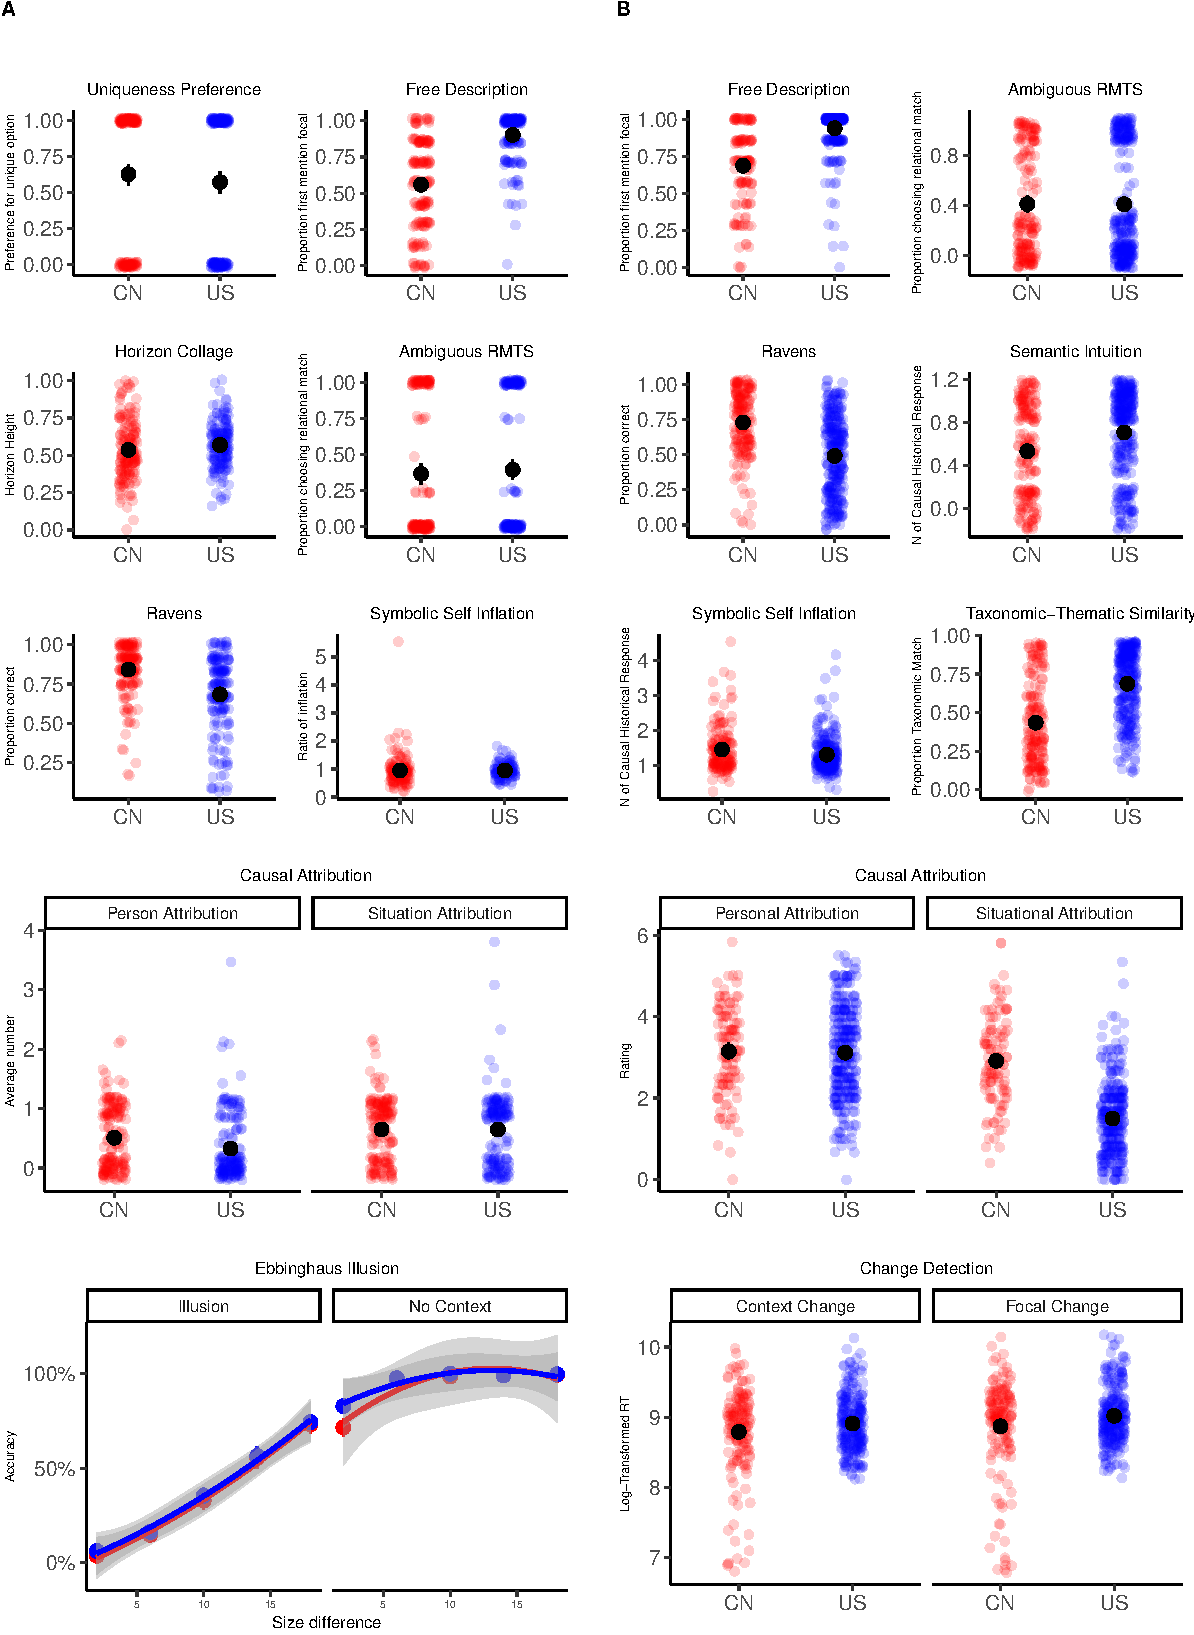
\includegraphics{visualization_files/figure-latex/unnamed-chunk-13-1.pdf}

\hypertarget{putting-d1-together}{%
\subsection{putting d1 together}\label{putting-d1-together}}

\begin{Shaded}
\begin{Highlighting}[]
\NormalTok{d1\_regular\_plot }\OtherTok{=}\NormalTok{ cowplot}\SpecialCharTok{::}\FunctionTok{plot\_grid}\NormalTok{(d1\_up\_plot, d1\_fd\_plot, d1\_hz\_plot, d1\_rmts\_plot, d1\_rv\_plot, d1\_ssi\_plot, }\AttributeTok{ncol =} \DecValTok{2}\NormalTok{)}
\NormalTok{d1\_wide\_plot }\OtherTok{=}\NormalTok{ cowplot}\SpecialCharTok{::}\FunctionTok{plot\_grid}\NormalTok{(d1\_ca\_plot, d1\_ebb\_plot, }\AttributeTok{ncol =} \DecValTok{1}\NormalTok{)}
\end{Highlighting}
\end{Shaded}

\begin{verbatim}
## Warning: Removed 1 rows containing non-finite values (stat_summary).
\end{verbatim}

\begin{verbatim}
## Warning: Removed 1 rows containing missing values (geom_point).
\end{verbatim}

\begin{Shaded}
\begin{Highlighting}[]
\NormalTok{d1\_all }\OtherTok{=} \FunctionTok{plot\_grid}\NormalTok{(d1\_regular\_plot, d1\_wide\_plot, }\AttributeTok{ncol =} \DecValTok{1}\NormalTok{, }\AttributeTok{greedy =} \ConstantTok{FALSE}\NormalTok{)}
\end{Highlighting}
\end{Shaded}

\hypertarget{fine-tuning-d2}{%
\section{fine tuning d2}\label{fine-tuning-d2}}

\hypertarget{non-generics-1}{%
\subsection{non generics}\label{non-generics-1}}

\hypertarget{cd}{%
\subsubsection{CD}\label{cd}}

\begin{Shaded}
\begin{Highlighting}[]
\NormalTok{raw\_CD }\OtherTok{\textless{}{-}}\NormalTok{ d2 }\SpecialCharTok{\%\textgreater{}\%} 
  \FunctionTok{filter}\NormalTok{(task\_name }\SpecialCharTok{==} \StringTok{"CD"}\NormalTok{) }\SpecialCharTok{\%\textgreater{}\%} 
  \FunctionTok{group\_by}\NormalTok{(subject, task\_info, culture) }\SpecialCharTok{\%\textgreater{}\%} 
  \FunctionTok{mutate}\NormalTok{(}\AttributeTok{resp =} \FunctionTok{log}\NormalTok{(}\FunctionTok{as.numeric}\NormalTok{(resp))) }\SpecialCharTok{\%\textgreater{}\%} 
  \FunctionTok{summarise}\NormalTok{(}\AttributeTok{mean\_log\_rt =} \FunctionTok{mean}\NormalTok{(resp, }\AttributeTok{na.rm =} \ConstantTok{TRUE}\NormalTok{)) }\SpecialCharTok{\%\textgreater{}\%} 
  \FunctionTok{mutate}\NormalTok{(}
         \AttributeTok{resp\_type\_print =} \FunctionTok{case\_when}\NormalTok{(}
\NormalTok{           task\_info }\SpecialCharTok{==} \StringTok{"context"} \SpecialCharTok{\textasciitilde{}} \StringTok{"Context Change"}\NormalTok{, }
           \ConstantTok{TRUE} \SpecialCharTok{\textasciitilde{}} \StringTok{"Focal Change"}
\NormalTok{         ))}
\end{Highlighting}
\end{Shaded}

\begin{verbatim}
## Warning in mask$eval_all_mutate(quo): NAs introduced by coercion

## Warning in mask$eval_all_mutate(quo): NAs introduced by coercion

## Warning in mask$eval_all_mutate(quo): NAs introduced by coercion

## Warning in mask$eval_all_mutate(quo): NAs introduced by coercion

## Warning in mask$eval_all_mutate(quo): NAs introduced by coercion

## Warning in mask$eval_all_mutate(quo): NAs introduced by coercion

## Warning in mask$eval_all_mutate(quo): NAs introduced by coercion

## Warning in mask$eval_all_mutate(quo): NAs introduced by coercion

## Warning in mask$eval_all_mutate(quo): NAs introduced by coercion

## Warning in mask$eval_all_mutate(quo): NAs introduced by coercion

## Warning in mask$eval_all_mutate(quo): NAs introduced by coercion

## Warning in mask$eval_all_mutate(quo): NAs introduced by coercion

## Warning in mask$eval_all_mutate(quo): NAs introduced by coercion

## Warning in mask$eval_all_mutate(quo): NAs introduced by coercion

## Warning in mask$eval_all_mutate(quo): NAs introduced by coercion

## Warning in mask$eval_all_mutate(quo): NAs introduced by coercion

## Warning in mask$eval_all_mutate(quo): NAs introduced by coercion

## Warning in mask$eval_all_mutate(quo): NAs introduced by coercion

## Warning in mask$eval_all_mutate(quo): NAs introduced by coercion

## Warning in mask$eval_all_mutate(quo): NAs introduced by coercion

## Warning in mask$eval_all_mutate(quo): NAs introduced by coercion

## Warning in mask$eval_all_mutate(quo): NAs introduced by coercion

## Warning in mask$eval_all_mutate(quo): NAs introduced by coercion

## Warning in mask$eval_all_mutate(quo): NAs introduced by coercion

## Warning in mask$eval_all_mutate(quo): NAs introduced by coercion

## Warning in mask$eval_all_mutate(quo): NAs introduced by coercion

## Warning in mask$eval_all_mutate(quo): NAs introduced by coercion

## Warning in mask$eval_all_mutate(quo): NAs introduced by coercion

## Warning in mask$eval_all_mutate(quo): NAs introduced by coercion

## Warning in mask$eval_all_mutate(quo): NAs introduced by coercion

## Warning in mask$eval_all_mutate(quo): NAs introduced by coercion

## Warning in mask$eval_all_mutate(quo): NAs introduced by coercion

## Warning in mask$eval_all_mutate(quo): NAs introduced by coercion

## Warning in mask$eval_all_mutate(quo): NAs introduced by coercion

## Warning in mask$eval_all_mutate(quo): NAs introduced by coercion

## Warning in mask$eval_all_mutate(quo): NAs introduced by coercion

## Warning in mask$eval_all_mutate(quo): NAs introduced by coercion

## Warning in mask$eval_all_mutate(quo): NAs introduced by coercion

## Warning in mask$eval_all_mutate(quo): NAs introduced by coercion

## Warning in mask$eval_all_mutate(quo): NAs introduced by coercion

## Warning in mask$eval_all_mutate(quo): NAs introduced by coercion

## Warning in mask$eval_all_mutate(quo): NAs introduced by coercion

## Warning in mask$eval_all_mutate(quo): NAs introduced by coercion

## Warning in mask$eval_all_mutate(quo): NAs introduced by coercion

## Warning in mask$eval_all_mutate(quo): NAs introduced by coercion

## Warning in mask$eval_all_mutate(quo): NAs introduced by coercion

## Warning in mask$eval_all_mutate(quo): NAs introduced by coercion

## Warning in mask$eval_all_mutate(quo): NAs introduced by coercion

## Warning in mask$eval_all_mutate(quo): NAs introduced by coercion

## Warning in mask$eval_all_mutate(quo): NAs introduced by coercion

## Warning in mask$eval_all_mutate(quo): NAs introduced by coercion

## Warning in mask$eval_all_mutate(quo): NAs introduced by coercion

## Warning in mask$eval_all_mutate(quo): NAs introduced by coercion

## Warning in mask$eval_all_mutate(quo): NAs introduced by coercion

## Warning in mask$eval_all_mutate(quo): NAs introduced by coercion

## Warning in mask$eval_all_mutate(quo): NAs introduced by coercion

## Warning in mask$eval_all_mutate(quo): NAs introduced by coercion

## Warning in mask$eval_all_mutate(quo): NAs introduced by coercion

## Warning in mask$eval_all_mutate(quo): NAs introduced by coercion
\end{verbatim}

\begin{verbatim}
## `summarise()` has grouped output by 'subject', 'task_info'. You can override
## using the `.groups` argument.
\end{verbatim}

\begin{Shaded}
\begin{Highlighting}[]
\NormalTok{d2\_cd\_plot }\OtherTok{\textless{}{-}} \FunctionTok{ggplot}\NormalTok{(}\AttributeTok{data =}\NormalTok{ raw\_CD, }
       \FunctionTok{aes}\NormalTok{(}\AttributeTok{y =}\NormalTok{ mean\_log\_rt, }\AttributeTok{x =}\NormalTok{ culture, }\AttributeTok{color =}\NormalTok{ culture)) }\SpecialCharTok{+}
\FunctionTok{geom\_point}\NormalTok{(}\AttributeTok{alpha =}\NormalTok{ .}\DecValTok{2}\NormalTok{, }\AttributeTok{position =} \FunctionTok{position\_jitter}\NormalTok{(}\AttributeTok{width =}\NormalTok{ .}\DecValTok{1}\NormalTok{)) }\SpecialCharTok{+} 
                    \FunctionTok{stat\_summary}\NormalTok{(}\AttributeTok{fun.data =} \StringTok{"mean\_cl\_boot"}\NormalTok{, }\AttributeTok{color =} \StringTok{"black"}\NormalTok{)}\SpecialCharTok{+}
\FunctionTok{scale\_color\_manual}\NormalTok{(}\AttributeTok{values =} \FunctionTok{c}\NormalTok{(}\StringTok{"red"}\NormalTok{, }\StringTok{"blue"}\NormalTok{))}\SpecialCharTok{+}
\FunctionTok{guides}\NormalTok{(}\AttributeTok{fill =} \StringTok{"none"}\NormalTok{) }\SpecialCharTok{+}
\FunctionTok{guides}\NormalTok{(}\AttributeTok{color =} \StringTok{"none"}\NormalTok{) }\SpecialCharTok{+}
\FunctionTok{ylab}\NormalTok{(}\StringTok{"Log{-}Transformed RT"}\NormalTok{) }\SpecialCharTok{+} 
\FunctionTok{xlab}\NormalTok{(}\StringTok{""}\NormalTok{)}\SpecialCharTok{+}
\FunctionTok{theme\_classic}\NormalTok{() }\SpecialCharTok{+}
  \FunctionTok{facet\_wrap}\NormalTok{(}\SpecialCharTok{\textasciitilde{}}\NormalTok{resp\_type\_print)}\SpecialCharTok{+}
  \FunctionTok{labs}\NormalTok{(}\AttributeTok{title =} \StringTok{"Change Detection"}\NormalTok{)  }\SpecialCharTok{+} 
  \FunctionTok{theme}\NormalTok{(}\AttributeTok{text =} \FunctionTok{element\_text}\NormalTok{(}\AttributeTok{size=}\DecValTok{4}\NormalTok{),}
      \AttributeTok{plot.title =} \FunctionTok{element\_text}\NormalTok{(}\AttributeTok{hjust =} \FloatTok{0.5}\NormalTok{, }\AttributeTok{size =} \DecValTok{8}\NormalTok{), }
      \AttributeTok{plot.subtitle =} \FunctionTok{element\_text}\NormalTok{(}\AttributeTok{hjust =} \FloatTok{0.5}\NormalTok{, }\AttributeTok{size =} \DecValTok{6}\NormalTok{))  }
\end{Highlighting}
\end{Shaded}

\hypertarget{causal-attribution}{%
\subsubsection{Causal Attribution}\label{causal-attribution}}

\begin{Shaded}
\begin{Highlighting}[]
\NormalTok{raw\_CA }\OtherTok{\textless{}{-}}\NormalTok{ d2 }\SpecialCharTok{\%\textgreater{}\%} 
  \FunctionTok{filter}\NormalTok{(task\_name }\SpecialCharTok{==} \StringTok{"CA"}\NormalTok{) }\SpecialCharTok{\%\textgreater{}\%} 
  \FunctionTok{group\_by}\NormalTok{(subject, task\_info, culture) }\SpecialCharTok{\%\textgreater{}\%} 
  \FunctionTok{mutate}\NormalTok{(}\AttributeTok{resp =}\NormalTok{ (}\FunctionTok{as.numeric}\NormalTok{(resp))) }\SpecialCharTok{\%\textgreater{}\%} 
  \FunctionTok{summarise}\NormalTok{(}\AttributeTok{mean\_resp =} \FunctionTok{mean}\NormalTok{(resp, }\AttributeTok{na.rm =} \ConstantTok{TRUE}\NormalTok{)) }\SpecialCharTok{\%\textgreater{}\%} 
  \FunctionTok{mutate}\NormalTok{(}
         \AttributeTok{resp\_type\_print =} \FunctionTok{case\_when}\NormalTok{(}
\NormalTok{           task\_info }\SpecialCharTok{==} \StringTok{"personal"} \SpecialCharTok{\textasciitilde{}} \StringTok{"Personal Attribution"}\NormalTok{, }
           \ConstantTok{TRUE} \SpecialCharTok{\textasciitilde{}} \StringTok{"Situational Attribution"}
\NormalTok{         ))}
\end{Highlighting}
\end{Shaded}

\begin{verbatim}
## `summarise()` has grouped output by 'subject', 'task_info'. You can override
## using the `.groups` argument.
\end{verbatim}

\begin{Shaded}
\begin{Highlighting}[]
\NormalTok{d2\_ca\_plot }\OtherTok{\textless{}{-}} \FunctionTok{ggplot}\NormalTok{(}\AttributeTok{data =}\NormalTok{ raw\_CA, }
       \FunctionTok{aes}\NormalTok{(}\AttributeTok{y =}\NormalTok{ mean\_resp, }\AttributeTok{x =}\NormalTok{ culture, }\AttributeTok{color =}\NormalTok{ culture)) }\SpecialCharTok{+}
\FunctionTok{geom\_point}\NormalTok{(}\AttributeTok{alpha =}\NormalTok{ .}\DecValTok{2}\NormalTok{, }\AttributeTok{position =} \FunctionTok{position\_jitter}\NormalTok{(}\AttributeTok{width =}\NormalTok{ .}\DecValTok{1}\NormalTok{)) }\SpecialCharTok{+} 
                    \FunctionTok{stat\_summary}\NormalTok{(}\AttributeTok{fun.data =} \StringTok{"mean\_cl\_boot"}\NormalTok{, }\AttributeTok{color =} \StringTok{"black"}\NormalTok{)}\SpecialCharTok{+}
\FunctionTok{scale\_color\_manual}\NormalTok{(}\AttributeTok{values =} \FunctionTok{c}\NormalTok{(}\StringTok{"red"}\NormalTok{, }\StringTok{"blue"}\NormalTok{))}\SpecialCharTok{+}
\FunctionTok{guides}\NormalTok{(}\AttributeTok{fill =} \StringTok{"none"}\NormalTok{) }\SpecialCharTok{+}
\FunctionTok{guides}\NormalTok{(}\AttributeTok{color =} \StringTok{"none"}\NormalTok{) }\SpecialCharTok{+}
\FunctionTok{ylab}\NormalTok{(}\StringTok{"Rating"}\NormalTok{) }\SpecialCharTok{+} 
\FunctionTok{xlab}\NormalTok{(}\StringTok{""}\NormalTok{)}\SpecialCharTok{+}
\FunctionTok{theme\_classic}\NormalTok{() }\SpecialCharTok{+}
  \FunctionTok{facet\_wrap}\NormalTok{(}\SpecialCharTok{\textasciitilde{}}\NormalTok{resp\_type\_print)}\SpecialCharTok{+}
  \FunctionTok{labs}\NormalTok{(}\AttributeTok{title =} \StringTok{"Causal Attribution"}\NormalTok{)  }\SpecialCharTok{+} 
  \FunctionTok{theme}\NormalTok{(}\AttributeTok{text =} \FunctionTok{element\_text}\NormalTok{(}\AttributeTok{size=}\DecValTok{4}\NormalTok{),}
      \AttributeTok{plot.title =} \FunctionTok{element\_text}\NormalTok{(}\AttributeTok{hjust =} \FloatTok{0.5}\NormalTok{, }\AttributeTok{size =} \DecValTok{8}\NormalTok{), }
      \AttributeTok{plot.subtitle =} \FunctionTok{element\_text}\NormalTok{(}\AttributeTok{hjust =} \FloatTok{0.5}\NormalTok{, }\AttributeTok{size =} \DecValTok{6}\NormalTok{)) }
\end{Highlighting}
\end{Shaded}

\hypertarget{generics-1}{%
\subsection{generics}\label{generics-1}}

\hypertarget{fd-1}{%
\subsubsection{FD}\label{fd-1}}

\begin{Shaded}
\begin{Highlighting}[]
\NormalTok{d2\_fd\_plot }\OtherTok{\textless{}{-}}\NormalTok{ d2\_base\_plot\_list}\SpecialCharTok{$}\NormalTok{FD }\SpecialCharTok{+} 
  \FunctionTok{ylab}\NormalTok{(}\StringTok{"Proportion first mention focal"}\NormalTok{) }\SpecialCharTok{+} 
  \FunctionTok{labs}\NormalTok{(}\AttributeTok{title =} \StringTok{"Free Description"}\NormalTok{)}

\NormalTok{d2\_fd\_plot}
\end{Highlighting}
\end{Shaded}

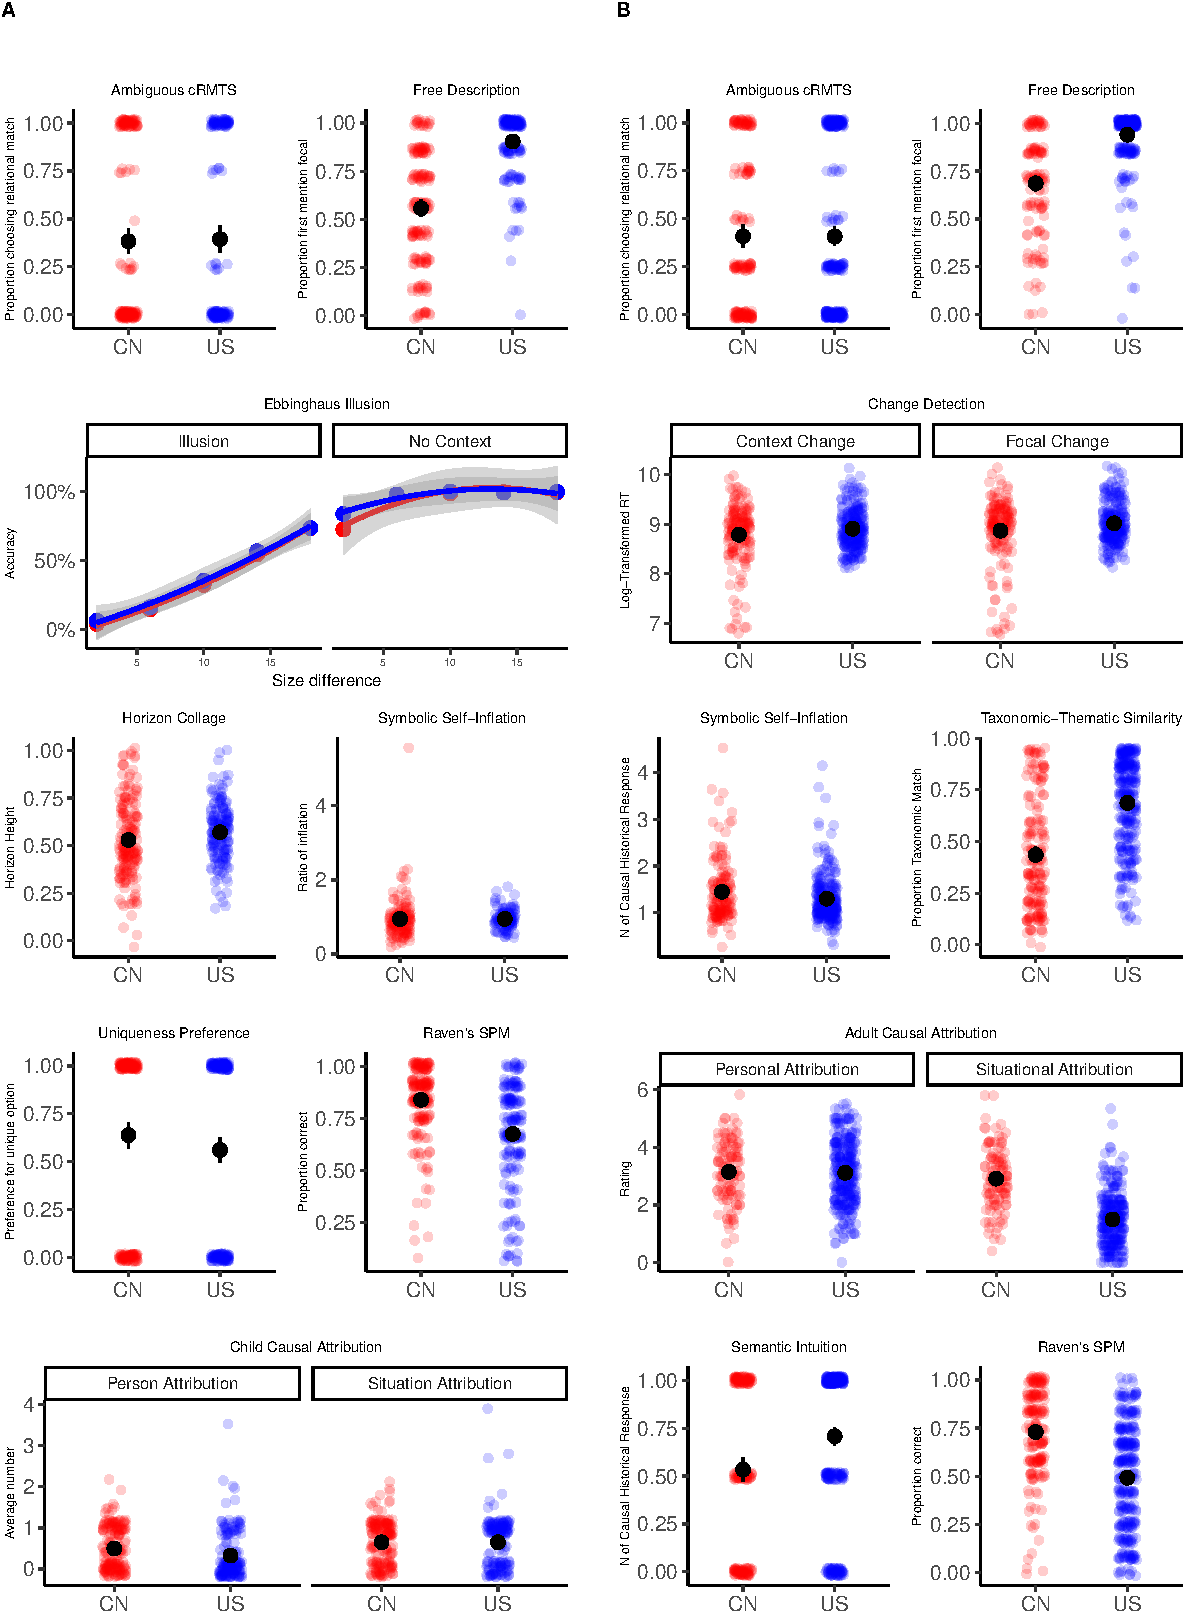
\includegraphics{visualization_files/figure-latex/unnamed-chunk-17-1.pdf}

\hypertarget{rmts-1}{%
\subsubsection{RMTS}\label{rmts-1}}

\begin{Shaded}
\begin{Highlighting}[]
\NormalTok{d2\_rmts\_plot }\OtherTok{\textless{}{-}}\NormalTok{ d2\_base\_plot\_list}\SpecialCharTok{$}\NormalTok{RMTS }\SpecialCharTok{+} 
  \FunctionTok{ylab}\NormalTok{(}\StringTok{"Proportion choosing relational match"}\NormalTok{) }\SpecialCharTok{+} 
  \FunctionTok{labs}\NormalTok{(}\AttributeTok{title =} \StringTok{"Ambiguous RMTS"}\NormalTok{)}
\NormalTok{d2\_rmts\_plot}
\end{Highlighting}
\end{Shaded}

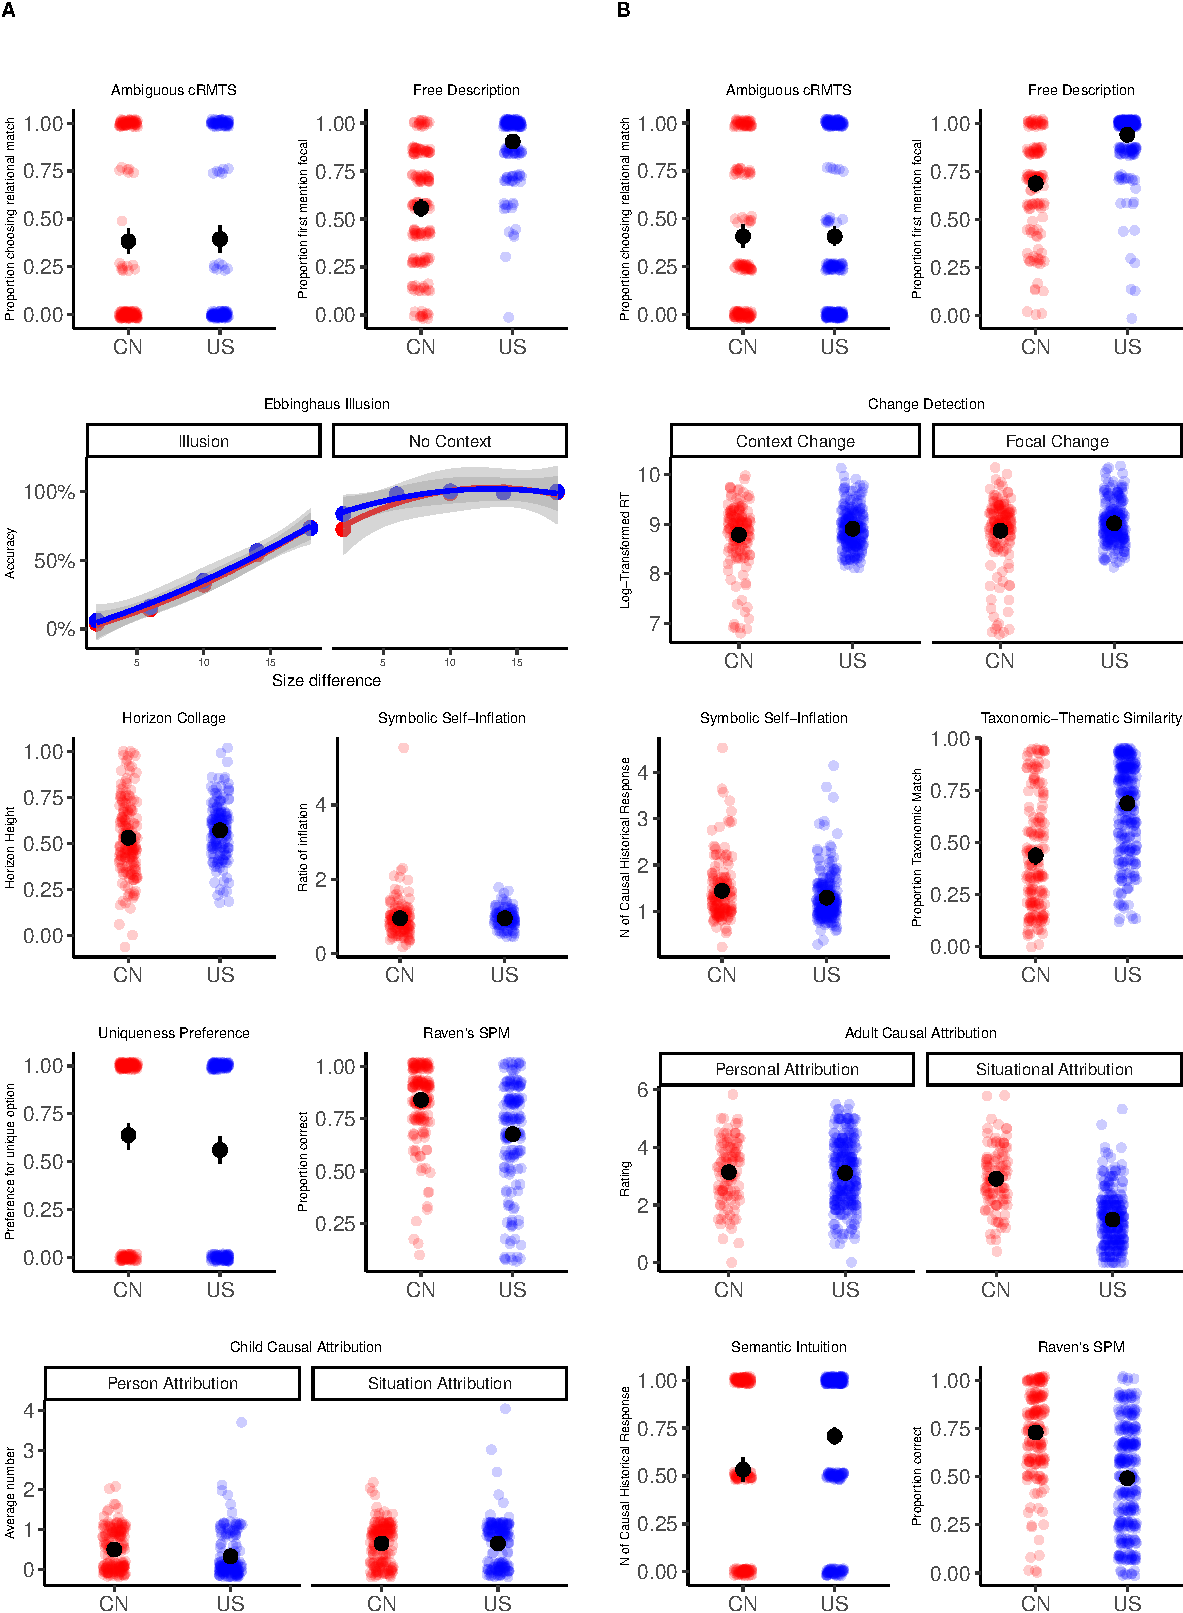
\includegraphics{visualization_files/figure-latex/unnamed-chunk-18-1.pdf}

\hypertarget{rv-1}{%
\subsubsection{RV}\label{rv-1}}

\begin{Shaded}
\begin{Highlighting}[]
\NormalTok{d2\_rv\_plot }\OtherTok{\textless{}{-}}\NormalTok{ d2\_base\_plot\_list}\SpecialCharTok{$}\NormalTok{RV }\SpecialCharTok{+} 
  \FunctionTok{ylab}\NormalTok{(}\StringTok{"Proportion correct"}\NormalTok{) }\SpecialCharTok{+} 
  \FunctionTok{labs}\NormalTok{(}\AttributeTok{title =} \StringTok{"Ravens"}\NormalTok{)}

\NormalTok{d2\_rv\_plot}
\end{Highlighting}
\end{Shaded}

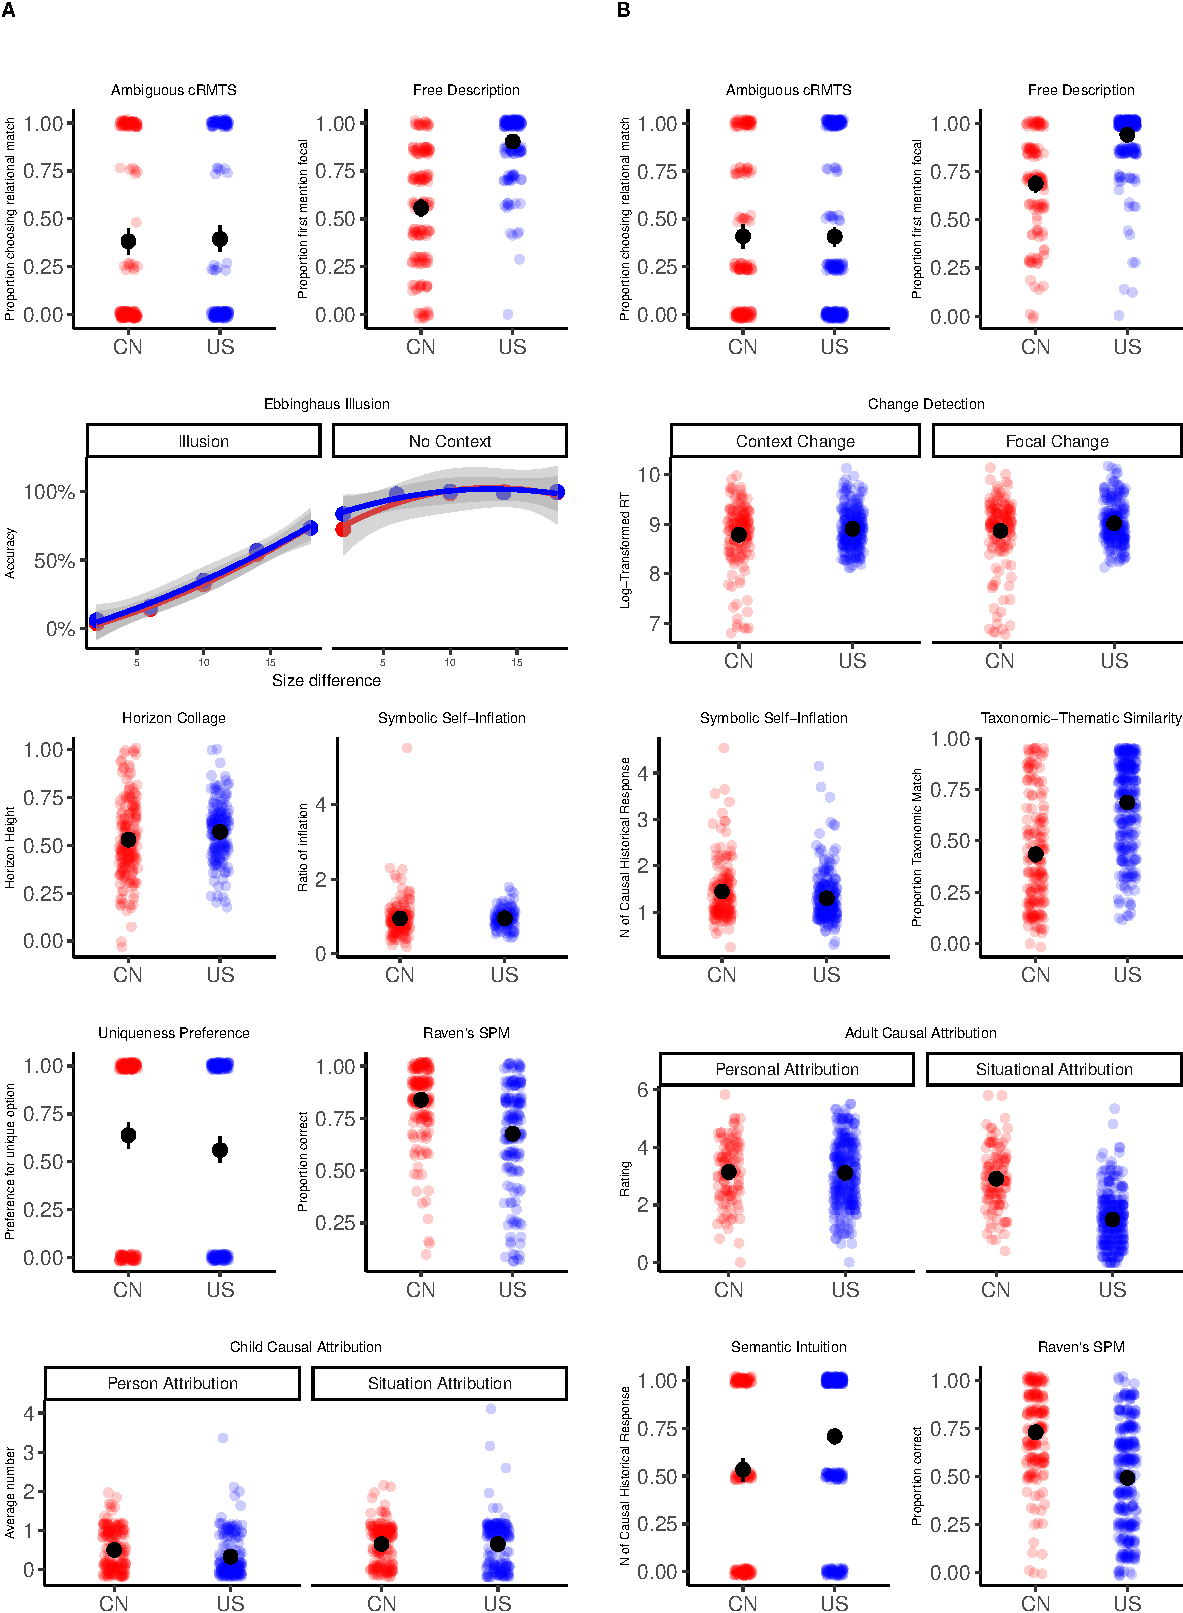
\includegraphics{visualization_files/figure-latex/unnamed-chunk-19-1.pdf}

\hypertarget{sei}{%
\subsubsection{SeI}\label{sei}}

\begin{Shaded}
\begin{Highlighting}[]
\NormalTok{d2\_sei\_plot }\OtherTok{\textless{}{-}}\NormalTok{ d2\_base\_plot\_list}\SpecialCharTok{$}\NormalTok{SeI }\SpecialCharTok{+} 
  \FunctionTok{ylab}\NormalTok{(}\StringTok{"N of Causal Historical Response"}\NormalTok{) }\SpecialCharTok{+} 
  \FunctionTok{labs}\NormalTok{(}\AttributeTok{title =} \StringTok{"Semantic Intuition"}\NormalTok{)}

\NormalTok{d2\_sei\_plot}
\end{Highlighting}
\end{Shaded}

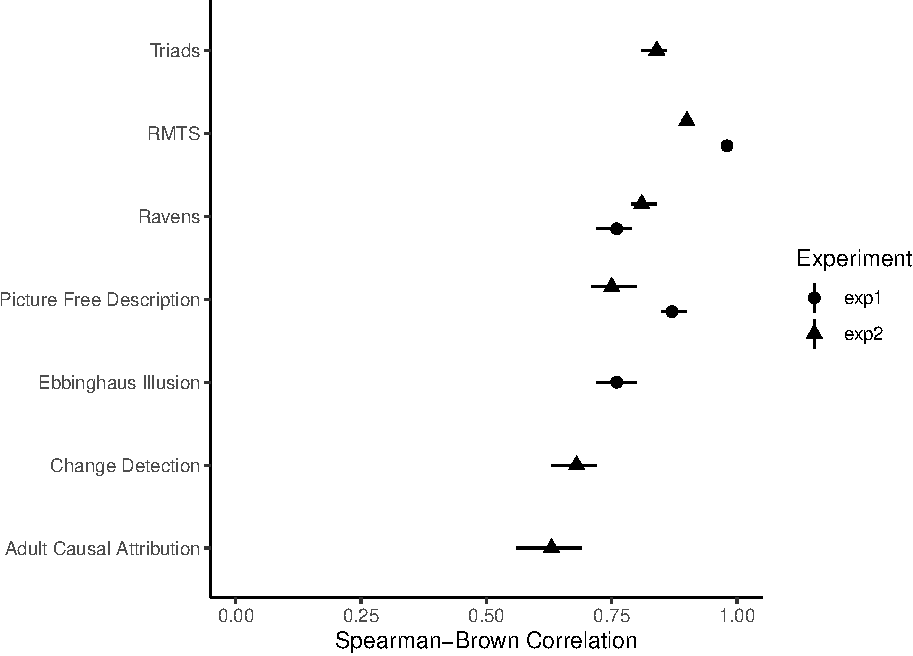
\includegraphics{visualization_files/figure-latex/unnamed-chunk-20-1.pdf}

\hypertarget{ssi}{%
\subsubsection{SSI}\label{ssi}}

\begin{Shaded}
\begin{Highlighting}[]
\NormalTok{d2\_ssi\_plot }\OtherTok{\textless{}{-}}\NormalTok{ d2\_base\_plot\_list}\SpecialCharTok{$}\NormalTok{SSI }\SpecialCharTok{+} 
  \FunctionTok{ylab}\NormalTok{(}\StringTok{"N of Causal Historical Response"}\NormalTok{) }\SpecialCharTok{+} 
  \FunctionTok{labs}\NormalTok{(}\AttributeTok{title =} \StringTok{"Symbolic Self Inflation"}\NormalTok{)}
\NormalTok{d2\_ssi\_plot}
\end{Highlighting}
\end{Shaded}

\includegraphics{visualization_files/figure-latex/unnamed-chunk-21-1.pdf}

\hypertarget{td}{%
\subsubsection{TD}\label{td}}

\begin{Shaded}
\begin{Highlighting}[]
\NormalTok{d2\_td\_plot }\OtherTok{\textless{}{-}}\NormalTok{ d2\_base\_plot\_list}\SpecialCharTok{$}\NormalTok{TD }\SpecialCharTok{+} 
  \FunctionTok{ylab}\NormalTok{(}\StringTok{"Proportion Taxonomic Match"}\NormalTok{) }\SpecialCharTok{+} 
  \FunctionTok{labs}\NormalTok{(}\AttributeTok{title =} \StringTok{"Taxonomic{-}Thematic Similarity "}\NormalTok{)}
\NormalTok{d2\_td\_plot}
\end{Highlighting}
\end{Shaded}

\includegraphics{visualization_files/figure-latex/unnamed-chunk-22-1.pdf}

\hypertarget{putting-d2-together}{%
\subsection{putting d2 together}\label{putting-d2-together}}

\begin{Shaded}
\begin{Highlighting}[]
\NormalTok{d2\_regular\_plot }\OtherTok{=}\NormalTok{ cowplot}\SpecialCharTok{::}\FunctionTok{plot\_grid}\NormalTok{(d2\_fd\_plot,d2\_rmts\_plot,d2\_rv\_plot,}
\NormalTok{                                     d2\_sei\_plot, d2\_ssi\_plot, d2\_td\_plot, }\AttributeTok{ncol =} \DecValTok{2}\NormalTok{)}
\NormalTok{d2\_wide\_plot }\OtherTok{=}\NormalTok{ cowplot}\SpecialCharTok{::}\FunctionTok{plot\_grid}\NormalTok{(d2\_ca\_plot, d2\_cd\_plot, }\AttributeTok{ncol =} \DecValTok{1}\NormalTok{)}

\NormalTok{d2\_all }\OtherTok{=} \FunctionTok{plot\_grid}\NormalTok{(d2\_regular\_plot, d2\_wide\_plot, }\AttributeTok{ncol =} \DecValTok{1}\NormalTok{)}
\end{Highlighting}
\end{Shaded}

\hypertarget{everything-togehter}{%
\section{everything togehter}\label{everything-togehter}}

\begin{Shaded}
\begin{Highlighting}[]
\CommentTok{\#}
\FunctionTok{plot\_grid}\NormalTok{(d1\_all, d2\_all, }\AttributeTok{labels =} \FunctionTok{c}\NormalTok{(}\StringTok{"Exp.1"}\NormalTok{, }\StringTok{"Exp.2"}\NormalTok{), }\AttributeTok{label\_size =} \DecValTok{10}\NormalTok{, }\AttributeTok{axis =} \StringTok{"r"}\NormalTok{)}
\end{Highlighting}
\end{Shaded}

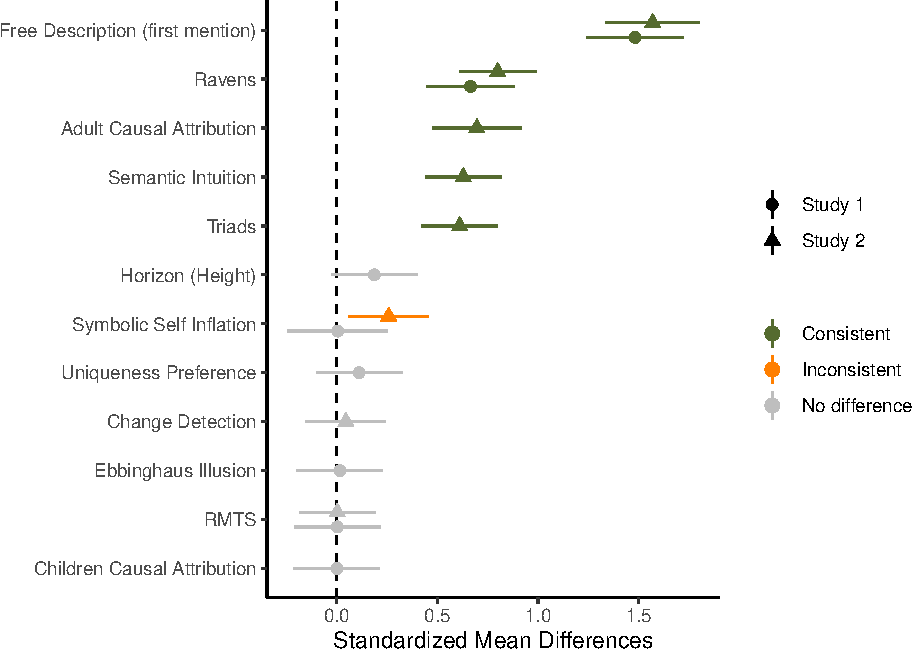
\includegraphics{visualization_files/figure-latex/unnamed-chunk-24-1.pdf}

\end{document}
